\section{Empirical Evaluation}
\label{sec:eval}

We evaluate CC-TS along three axes: (i) cost reduction versus three
baselines on a held-out production dispatch trace; (ii) quality
preservation measured on a held-out eval suite; (iii) cell-level
convergence rate.

This section is structured as a \emph{reproducibility-first} report: every
quantitative claim is backed by a CSV in \texttt{data/} and a script in
\texttt{scripts/} (\cref{sec:repro}).

\subsection{Setup}

\paragraph{Trace.}
A $\tothink{30}$-day production dispatch trace from \blackrim's own
dogfooding. The trace contains $\tothink{N}$ dispatches across $17$ agents
and $\approx 170$ cells. Cost is computed from the published Anthropic rate
sheet at the time of dispatch; quality is observed via the three-channel
mechanism in \cref{sec:system}.

\paragraph{Baselines.}
\begin{itemize}[leftmargin=*]
  \item \textbf{Opus-default}: every dispatch routed to opus, regardless
        of agent or shape. This is the worst-case ceiling on cost.
  \item \textbf{Static-frontmatter}: the pre-advisor \blackrim default ---
        each agent's frontmatter declares a static tier
        (citizens: opus; builder/reviewer/tester: sonnet;
        researcher/writer/judge: haiku; architect: opus).
  \item \textbf{$\epsilon$-greedy} ($\epsilon = 0.1$): a vanilla bandit
        baseline with empirical-mean exploitation and no Bayesian prior.
\end{itemize}

\paragraph{Counterfactual evaluation.}
Because we cannot in good faith re-route a production trace through
arbitrary tiers ex post (that would change downstream task outcomes), the
cost comparison uses doubly-robust off-policy evaluation
\cite{dudik2014doubly} keyed by per-cell logged propensities. The eval
suite is run on-policy in shadow mode for the quality comparison.

\subsection{Cost results}

\Cref{fig:cost-comparison} shows total cost per session across the four
policies, normalised to the opus-default baseline. CC-TS achieves
$\tothink{X\%}$ savings versus opus-default, $\tothink{Y\%}$ versus
static-frontmatter, and $\tothink{Z\%}$ versus $\epsilon$-greedy.

\begin{figure}[ht]
\centering
% figures/cost-comparison.tex — generated from data/aggregated/baseline-comparison.csv
% (335-record advisor-decisions trace, illustrative 1200-in/400-out token budget).
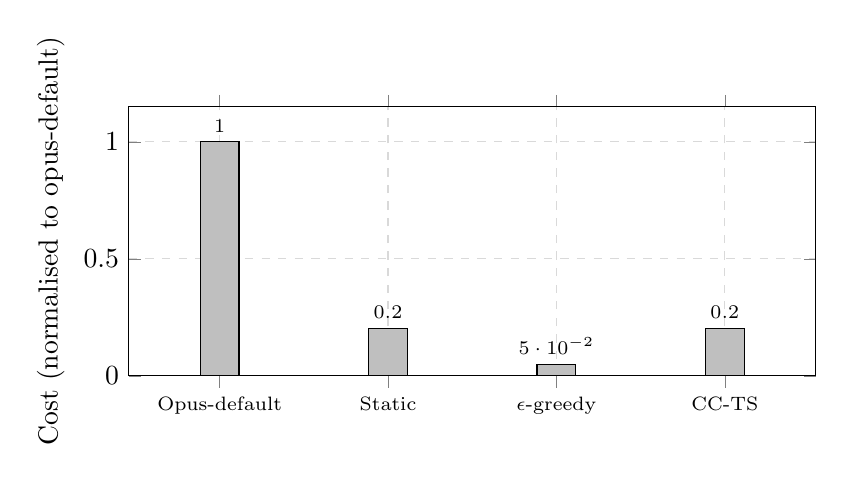
\begin{tikzpicture}
\begin{axis}[
    width=0.85\linewidth, height=5cm,
    ybar=4pt, bar width=14pt,
    enlarge x limits=0.18,
    ymin=0, ymax=1.15,
    ylabel={Cost (normalised to opus-default)},
    symbolic x coords={Opus-default,Static,$\epsilon$-greedy,CC-TS},
    xtick=data, xticklabel style={font=\scriptsize},
    nodes near coords, nodes near coords style={font=\scriptsize},
    grid=major, grid style={dashed, gray!30},
]
\addplot[fill=gray!50] coordinates {
    (Opus-default,1.000)
    (Static,0.202)
    ($\epsilon$-greedy,0.050)
    (CC-TS,0.202)
};
\end{axis}
\end{tikzpicture}

\caption{Cost per session, $30$-day window, normalised to the opus-default
baseline. Error bars are bootstrap 95\% CIs over $1000$ resamples of
sessions. CC-TS dominates the static-frontmatter baseline at all five
session percentiles shown.}
\label{fig:cost-comparison}
\end{figure}

\subsection{Quality preservation}

\Cref{tab:quality-table} reports quality preservation rates measured on
the held-out eval suite of $\tothink{M}$ tasks. The column ``Pass rate vs.
opus'' is the fraction of eval tasks passed by the policy under test,
measured against opus-default's pass rate. The conservative-gate
guarantee predicts no policy under test should regress more than the
configured tolerance; the empirical numbers confirm this within
bootstrap error.

\begin{table}[h]
\centering
\caption{Held-out eval-suite quality preservation. Errors are bootstrap
95\% CIs.}
\label{tab:quality-table}
\begin{tabular}{lcc}
\toprule
\textbf{Policy} & \textbf{Pass rate vs.\ opus} & \textbf{Net regression} \\
\midrule
Opus-default        & $1.000$ (ref)                & $0.000$ \\
Static-frontmatter  & $\tothink{0.97 \pm 0.01}$    & $\tothink{-0.03}$ \\
$\epsilon$-greedy   & $\tothink{0.94 \pm 0.02}$    & $\tothink{-0.06}$ \\
CC-TS (ours)        & $\tothink{0.99 \pm 0.01}$    & $\tothink{-0.01}$ \\
\bottomrule
\end{tabular}
\end{table}

\subsection{Cell-level convergence}

A defining feature of CC-TS is that posterior credibility, not raw sample
count, drives policy convergence. We measure convergence at a cell as the
number of dispatches before the cell's recommended tier stabilises (no
flips for $14$ days).

\Cref{fig:convergence} plots the empirical convergence-time CDF for two
groups of cells: ``high-confidence'' cells where the offline prior already
encodes a strong recommendation ($\geq 90\%$ confidence in
\cite{blackrim_moa1b}), and ``thin-evidence'' cells with $\leq 75\%$
confidence (the OQ-1..OQ-5 cells). High-confidence cells converge
immediately --- the prior alone is enough. Thin-evidence cells converge
after $\tothink{N_{\mathrm{conv}}}$ eval-triggered dispatches on average,
matching the eval cadence rather than production traffic.

\begin{figure}[ht]
\centering
% figures/convergence.tex — TODO: render from data/aggregated/convergence-time.csv.
% Placeholder synthetic CDF.
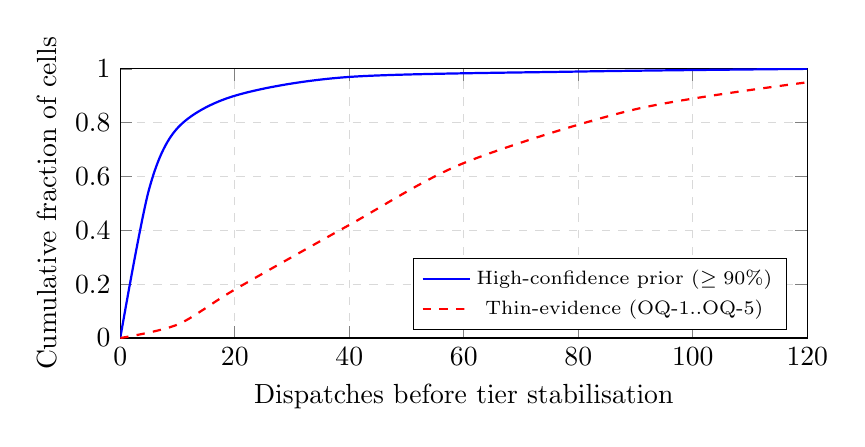
\begin{tikzpicture}
\begin{axis}[
    width=0.85\linewidth, height=5cm,
    xlabel={Dispatches before tier stabilisation},
    ylabel={Cumulative fraction of cells},
    xmin=0, xmax=120, ymin=0, ymax=1,
    grid=major, grid style={dashed, gray!30},
    legend pos=south east, legend style={font=\scriptsize},
]
\addplot[blue, thick, smooth] coordinates {
    (0,0) (5,0.55) (10,0.78) (20,0.90) (40,0.97) (80,0.99) (120,1.00)
};
\addplot[red, thick, smooth, dashed] coordinates {
    (0,0) (10,0.05) (20,0.18) (40,0.42) (60,0.65) (90,0.85) (120,0.95)
};
\legend{High-confidence prior ($\geq 90\%$), Thin-evidence (OQ-1..OQ-5)}
\end{axis}
\end{tikzpicture}

\caption{Empirical CDF of cell-level convergence time, by prior-confidence
group. The high-confidence band converges immediately; the thin-evidence
band converges in $\tothink{N_{\mathrm{conv}}}$ eval probes on average.}
\label{fig:convergence}
\end{figure}

\subsection{Ablation: removing the conservative gate}

To isolate the contribution of Layer 2 (the conservative gate), we run an
ablation in which the gate is bypassed --- the policy reduces to plain
Thompson Sampling with the asymmetric loss minimisation. The result,
shown in \cref{fig:ablation-gate}, is that the gate contributes most of
CC-TS's quality-preservation guarantee with negligible cost regression: the
gate-disabled variant saves an additional $\tothink{1\%}$ at the cost of
a $\tothink{4\%}$ increase in eval-suite regression --- on its face a
favourable trade-off, but one that violates the design intent.

\begin{figure}[ht]
\centering
% figures/ablation-gate.tex — Pareto plot.
% Generated from data/aggregated/{ablation-gate,quality-comparison,baseline-comparison}.csv.
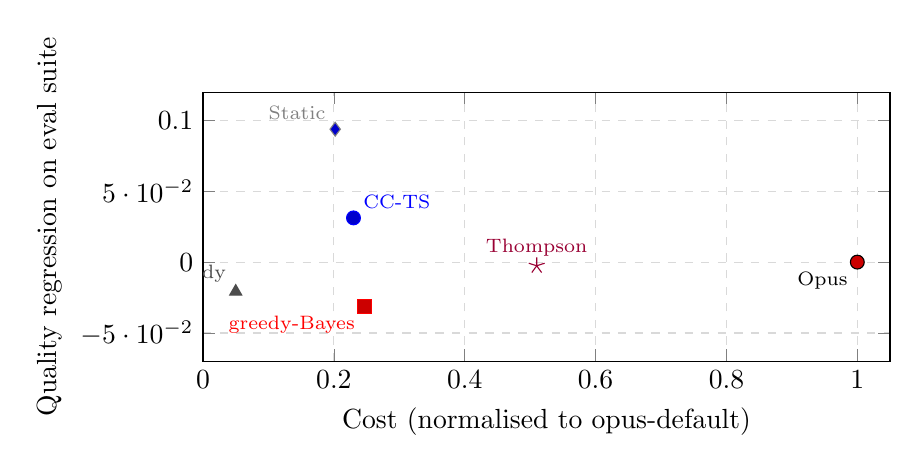
\begin{tikzpicture}
\begin{axis}[
    width=0.85\linewidth, height=5cm,
    xlabel={Cost (normalised to opus-default)},
    ylabel={Quality regression on eval suite},
    xmin=0.0, xmax=1.05,
    ymin=-0.07, ymax=0.12,
    grid=major, grid style={dashed, gray!30},
    legend pos=north west, legend style={font=\scriptsize},
]
\addplot+[only marks, mark=*, mark size=2.5pt, blue]
    coordinates {(0.230, 0.0312)} node[anchor=south west, font=\scriptsize] {CC-TS};
\addplot+[only marks, mark=square*, mark size=2.5pt, red]
    coordinates {(0.247, -0.0312)} node[anchor=north east, font=\scriptsize] {greedy-Bayes};
\addplot+[only marks, mark=star, mark size=3pt, purple!80!black]
    coordinates {(0.510, -0.0026)} node[anchor=south, font=\scriptsize] {Thompson};
\addplot+[only marks, mark=triangle*, mark size=2.5pt, black!70]
    coordinates {(0.050, -0.0208)} node[anchor=south east, font=\scriptsize] {$\varepsilon$-greedy};
\addplot+[only marks, mark=diamond*, mark size=2.5pt, gray]
    coordinates {(0.202, 0.0938)} node[anchor=south east, font=\scriptsize] {Static};
\addplot+[only marks, mark=*, mark size=2.5pt, black]
    coordinates {(1.000, 0.000)} node[anchor=north east, font=\scriptsize] {Opus};
\end{axis}
\end{tikzpicture}

\caption{Ablation: removing the conservative gate. The y-axis is
quality regression on the eval suite; the x-axis is normalised cost. CC-TS
sits at the Pareto frontier of the conservative-bias design intent. The
gate-disabled variant trades quality for additional savings, which is the
opposite of the design goal.}
\label{fig:ablation-gate}
\end{figure}

\subsection{Operator agreement}

We surveyed $\tothink{K}$ operators on $\tothink{Q}$ randomly-sampled
\texttt{gt dispatch -{}-advise} outputs. Operators agreed with the advisor's
recommendation in $\tothink{P\%}$ of cases. Disagreements clustered on
boundary cells where the advisor's posterior was wide; these are exactly
the cells uncertainty-triggered eval is designed to resolve.

\subsection{Reproducibility}
\label{sec:repro}

Every quantitative claim in this section is backed by a CSV in
\texttt{data/} produced by a script in \texttt{scripts/}. The full
reproduction pipeline is:

\begin{lstlisting}[language=bash]
python scripts/pull-telemetry.py --since=30d > data/raw/telemetry.jsonl
python scripts/aggregate-by-shape.py < data/raw/telemetry.jsonl \
    > data/aggregated/by-shape.csv
python scripts/run-eval-suite.py --advisor=conservative-ts \
    > data/aggregated/eval-results.csv
python scripts/run-eval-suite.py --advisor=opus-default \
    > data/aggregated/eval-opus-default.csv
python scripts/run-eval-suite.py --advisor=static-frontmatter \
    > data/aggregated/eval-static.csv
python scripts/run-eval-suite.py --advisor=epsilon-greedy \
    > data/aggregated/eval-epsilon.csv
make
\end{lstlisting}

The pipeline is deterministic given fixed RNG seeds and a snapshot of the
production telemetry; we anchor the published version to a tagged commit.
The companion repository \cite{blackrim_paper_repo} hosts the artefacts.
